\section{Related Work}
\label{sec:precise-alignment-related-work}

The precise global localisation of a robotic platform within a vineyard environment can be broken down into three technical problems. First, the robot must generate detailed, metrically scaled three-dimensional representations of the vine and/or environment from its onboard sensors. Second, a global structural reference map must already exist against which those local observations can be compared. Third, reliable algorithms must compute the rigid transformation that aligns the local capture to the global frame, recovering the robot's pose with centimetric accuracy. This section reviews each problem as follows: proximal (close-range, ground-level) three-dimensional sensing via stereo, RGB-D, and LiDAR modalities; the construction of dense reference maps from LiDAR and photogrammetric pipelines; and the class of point cloud registration algorithms built upon the Iterative Closest Point (ICP) framework.

\subsection{Stereo Depth Imaging}
\label{subsec:stereo-depth}

Stereo and RGB-D imaging systems are widely used to generate three-dimensional models of individual plants. Depth is recovered from the disparity $d$ between corresponding pixels in a rectified stereo pair, related to metric depth $Z$ by the standard pinhole model equation:
%
\begin{equation}
    Z = \frac{f \cdot B}{d},
\end{equation}
%
where $f$ is the focal length and $B$ is the baseline between the two image sensors.

Klodt et al.~\cite{klodtFieldPhenotypingGrapevine2015} established that passive stereo cameras are sufficient for quantitative vine characterisation under realistic outdoor conditions, generating dense depth maps from paired RGB images without requiring a controlled background or calibration rig. Parr et al.~\cite{parrAnalysisDepthCameras2022} subsequently benchmarked five depth sensor modalities on grape clusters under both laboratory and open-field conditions, comparing structured light, active-infrared (IR) stereo, time-of-flight, and LiDAR-based sensors. Their results showed that the RealSense D415 active IR stereo sensor achieved approximately 2\,mm error in controlled indoor conditions and remained functional in full sunlight, whereas time-of-flight and structured-light sensors exhibited larger measurement bias. These comparative findings provide an empirical basis for depth sensor selection in precise mapping vineyard tasks. Active RGB-D sensors (e.g., Azure Kinect) offer artificial texture projection for feature-poor scenes but suffer systematic depth failures under direct sunlight~\cite{tolgyessyEvaluationAzureKinect2021}, making passive stereo the more practical modality for outdoor vineyard deployment.

More recently, foundation model approaches have been applied to stereo depth estimation with the goal of achieving reliable zero-shot generalisation across varied imaging conditions. FoundationStereo~\cite{wenFoundationStereoZeroShot2025}
addresses the sim-to-real transfer problem by training on a curated dataset of one million photorealistic synthetic stereo pairs and employing a Side-Tuning Adapter (STA) to leverage monocular depth priors from DepthAnything V2; cost volumes are subsequently filtered via an Attentive Hybrid Cost Filtering (AHCF) module combining Axial-Planar Convolutions with a Disparity Transformer for long-range disparity reasoning. The model demonstrates strong zero-shot generalisation across the Middlebury and ETH3D benchmarks, with a separately fine-tuned variant achieving state-of-the-art on ETH3D, and performs well on in-the-wild data, as illustrated in \cref{fig:zeroShotFS}. In the present work, FoundationStereo is applied to imagery from a ZED Mini stereo camera to produce the depth maps from which the source point cloud is derived prior to registration.

\begin{figure}[htbp]
    \centering
    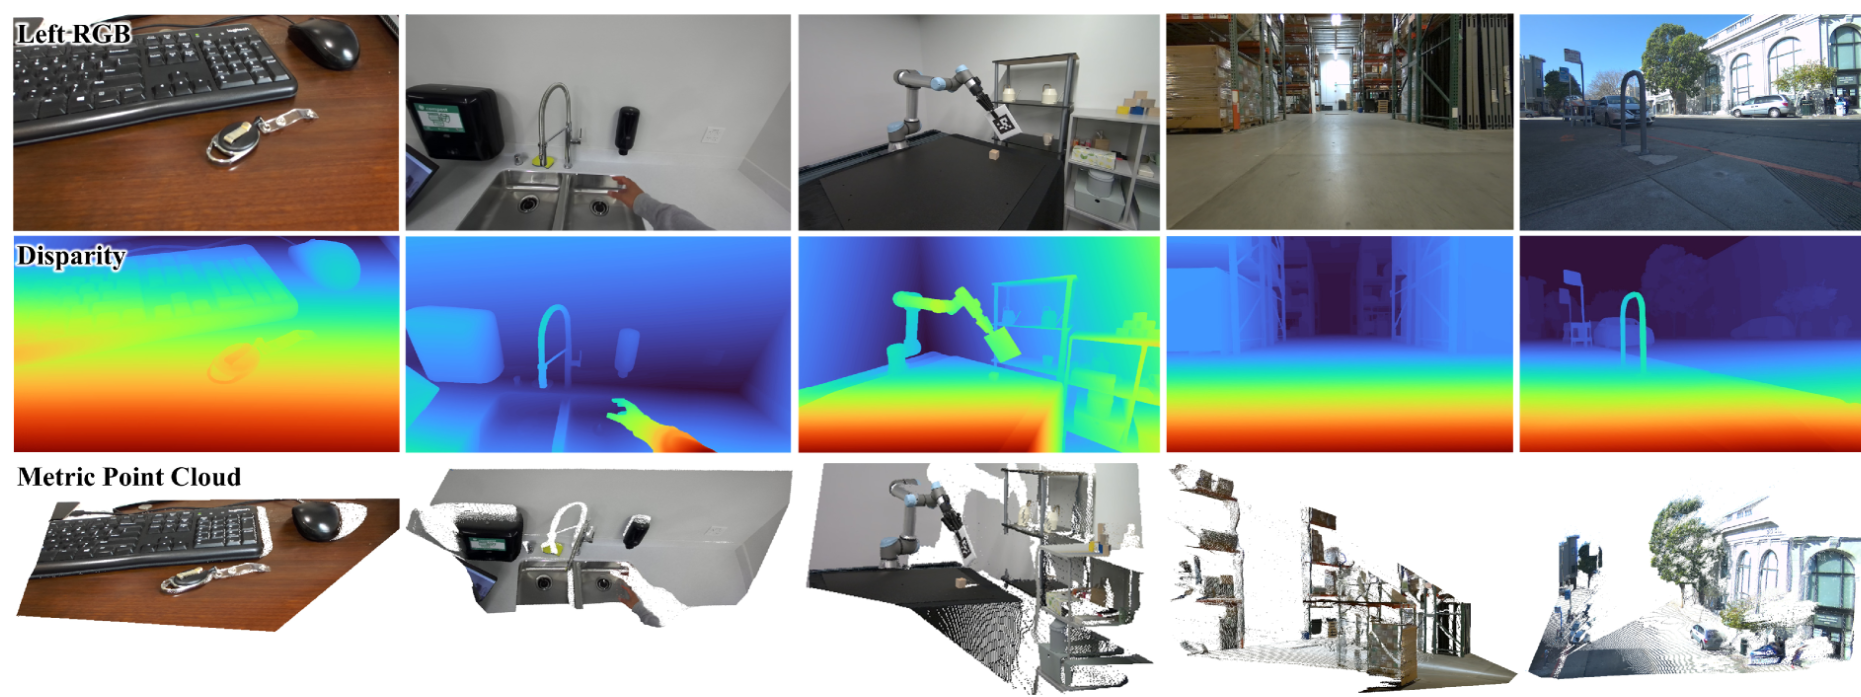
\includegraphics[width=0.9\linewidth]{4-precise-alignment/4-related-work/figures/zeroShotFSImages.png}
    \caption{Zero-shot stereo depth predictions from FoundationStereo across diverse in-the-wild scenes, including indoor and outdoor environments, textureless and reflective surfaces, and challenging illumination conditions. No per-domain fine-tuning is performed \protect\cite{wenFoundationStereoZeroShot2025}.}
    \label{fig:zeroShotFS}
\end{figure}

\subsection{Dense LiDAR Mapping}
\label{subsec:dense-lidar-mapping}

The preceding chapter employed LiDAR for real-time odometry and mapping; this subsection considers its complementary role in constructing the dense, 
centimetre-resolution reference models against which the robot subsequently localises. Unlike stereo imaging, LiDAR measures physical geometry rather than visual appearance and is therefore substantially more robust to scene texture variation; however, highly reflective, specular, or strongly light-absorbing surfaces can still produce erroneous returns, signal loss, or elevated noise in the resulting point cloud. LiDAR performs consistently during the dormant season when vine architecture is reduced to bare wood, which is precisely when precision pruning operations are carried out.

At the proximal sensing scale relevant to this thesis, Moreno et al.~\cite{morenoOnGroundVineyardReconstruction2020} demonstrated high-density 3D reconstruction of dormant vine rows using a downward-facing 2D time-of-flight LiDAR mounted on an electric platform georeferenced via RTK-GNSS. Applying $\alpha$-shape fitting to extract branch volumes, they reported a linear correlation with actual dry biomass of $R^2 = 0.85$, confirming that ground-level LiDAR produces geometrically faithful vine models at centimetre resolution. The sensor-to-canopy distances employed (0.5--1.5\,m) are comparable to the operating range evaluated in \cref{sec:precise-alignment-results}. Teng et al.~\cite{tengAccuracyEvaluationBranch2023} compared backpack-mounted 3D LiDAR SLAM against UAV-SfM for modelling dormant peach trees during winter pruning, finding that the ground-level LiDAR approach achieved higher geometric accuracy ($R^2 = 0.93$ against pruned branch fresh weight) with shorter acquisition time than the aerial photogrammetric alternative. Their results confirm that mobile LiDAR SLAM produces reference-quality models of bare-branch fruit tree structure at close range, and that branches with diameters exceeding 3\,cm are reliably resolved in the resulting point clouds.

Petrović et al.~\cite{petrovicVineCanopyReconstruction2022} directly compared terrestrial LiDAR and UAV photogrammetric reconstruction on defoliated vines, finding that both modalities achieve regression against ground-truth geometry of $R \approx 0.9$. This indicates that dense LiDAR-generated point clouds are a viable alternative to SfM for constructing global reference maps. The maps produced in that study span a survey area of 7\,m~$\times$~28\,m. Comparatively, the SfM-derived 3DGS reference map used in this thesis covers a single vineyard bay (three to four vines within the global ENU frame). 

No matter whether the real-time pointcloud model is created by a stereo camera or a LiDAR, the final alignment step requires a common algorithmic framework for registering the two point clouds.

\subsection{Point Cloud Registration}
\label{subsec:registration-methods}

The ICP algorithm and its foundational variants (point-to-plane and Generalised-ICP) were introduced in \cref{subsec:bg-point-cloud-registration}. This section reviews the broader landscape of registration methods that inform the design choices made in the precise-alignment pipeline.

Rusinkiewicz and Levoy~\cite{rusinkiewiczEfficientVariantsICP2001} provided an influential taxonomy of ICP design choices, classifying variants across point selection, correspondence matching, and minimisation strategy, and demonstrated that a well-chosen combination achieves alignment in a few tens of milliseconds. Huang et al.~\cite{huangComprehensiveSurveyPoint2021} surveyed both optimisation-based and deep learning registration methods, finding that optimisation-based approaches generalise well to novel scenes without training data, whereas learned methods degrade when the target scene differs from the training distribution. Their survey also identifies density difference and scale variation as the dominant challenges in cross-source registration, directly characterising the alignment problem in this thesis, where a dense stereo-derived point cloud must be registered against a photogrammetric reference model with fundamentally different density and noise characteristics.

Several extensions of ICP improve robustness in the geometrically repetitive, texturally ambiguous structure of vineyard rows. Beyond the Generalised-ICP formulation introduced in \cref{subsec:bg-point-cloud-registration}, which models local surface patches as Gaussian distributions and reduces sensitivity to incorrect correspondences, further variants augment the correspondence metric with additional geometric or photometric information. He et al.~\cite{heIterativeClosestPoints2017} proposed GF-ICP, a feature-augmented variant that incorporates point curvature, surface normals, and local density into the correspondence cost. This enriched error metric enables convergence from larger initial errors than pure geometric proximity allows. Choi et al.~\cite{choiIterativeKClosestPoint2020} extended ICP to coloured point clouds through a probabilistic K-closest matching formulation with a colour-supported objective, adding a photometric constraint that reduces correspondence ambiguity in regions with visually distinct surface texture, a useful property when aligning vine bark or cane surface reconstructions.

Semantic ICP, as developed by Chen et al.~\cite{chenSemanticICPIterativeClosest2025}, restricts correspondence matching to points sharing the same semantic class label. This prevents the structurally plausible but semantically incorrect matches. Vizzo et al.~\cite{vizzoKISSICPDefensePointtoPoint2023} demonstrated with KISS-ICP that a deliberately lean point-to-point formulation, augmented by adaptive correspondence thresholding and a robust kernel for outlier rejection, achieves competitive LiDAR odometry accuracy across diverse sensor platforms and environments without requiring per-deployment parameter tuning. Their finding that engineering simplicity can match or exceed more complex variants in practice has informed the design of several subsequent registration systems.

A fundamental limitation common to all ICP variants is sensitivity to the initial pose estimate: convergence to the global optimum of the ICP objective (\cref{eq:icp}) is not assured when the initial alignment error exceeds the geometric scale of distinctive scene features. For the more challenging case of global registration from an arbitrary initial pose, Mellado et al.~\cite{melladoSuper4PCSFastGlobal2014} introduced Super4PCS, which detects congruent four-point bases across two overlapping point clouds in linear time, enabling alignment in arbitrary initial orientations with as little as 25\% overlap. Yang et al.~\cite{yangGoICPGloballyOptimal2016} proposed Go-ICP, which employs a branch-and-bound search over the $SE(3)$ space of rigid transformations, guaranteeing globally optimal ICP solutions by systematically excluding sub-optimal rotation regions at the cost of increased computation.

The most recent direction adapts deep learning to replace hand-crafted descriptors with learned representations. Elbaz et al.~\cite{elbaz3DPointCloudRegistration2017} trained a deep auto-encoder to encode overlapping local regions of a point cloud into compact feature vectors; matched descriptor pairs initialise a subsequent ICP refinement, enabling robust alignment even under the large initial misalignment typical when registering a close-range scan against a large-scale prior map. Zhang et al.~\cite{zhangDeepLearningBased2020} provide a systematic review of deep learning-based registration methods, concluding that learned descriptors consistently outperform hand-crafted alternatives on standard benchmarks, in particular under noise and low-overlap conditions. Xu et al.~\cite{xuCross3DRegLargescaleRealworld2025} address the further challenge of cross-source registration, specifically aligning point clouds from heterogeneous sensor types, such as a spinning mechanical LiDAR and a semi-solid-state LiDAR, through a visual-geometric attention module that fuses image and geometric features to establish robust correspondences across point clouds with different density and pattern distributions. A global survey by Yin et al.~\cite{yinSurveyGlobalLiDAR2024} identifies the central open challenge in LiDAR-based global localisation as reliably retrieving the correct initial alignment hypothesis within a large-scale map, noting that the dominant operational approach (global place retrieval followed by local ICP refinement) remains fragile under seasonal appearance change, a challenge directly relevant to long-term autonomous deployment in vineyards.